%%%%%%%%%%%%%%%%%%%%%%%%%%%%%%%%%%%%%%%%%%%%%%%%%%%%%%%%%%%%%%%%%%%%%%%%
%                                                                      %
%     File: Thesis_Results.tex                                         %
%     Tex Master: Thesis.tex                                           %
%                                                                      %
%     Author: Andre C. Marta                                           %
%     Last modified : 29 Jan 2021                                      %
%                                                                      %
%%%%%%%%%%%%%%%%%%%%%%%%%%%%%%%%%%%%%%%%%%%%%%%%%%%%%%%%%%%%%%%%%%%%%%%%

\chapter{Proposta de Arquitectura}
\label{chapter:results}

A arquitectura de um dispositivo deve ser cuidadosamente fundamentada num conjunto de metas que se pretendem assegurar, definindo as melhores estratégias para as cumprir o melhor que se possa com os recursos disponíveis. Neste trabalho decidiu-se que o mais importante seria procurar ao máximo assegurar a transmissão de todas as tramas que se apresentem ao dispositivo, tal como a correta execução do PTP. De modo que não ocorram situações em que o comutador tenha que descartar uma dada trama em detrimento de outras, é necessário que a arquitectura escolhida seja capaz de transmitir tramas com o mesmo débito com que as recebe. No entanto, devido ao estágio inicial em que se encontra o projeto no qual se insere este trabalho, ainda não há conhecimento das características das redes em que este dispositivo possa ser inserido. Assim, tentar-se-à maximizar o débito no dispositivo de acordo com o tempo disponível para a elaboração do mesmo. 


\section{\textit{Switch fabric}}


Como discutido no capítulo anterior, o débito num comutador é, essencialmente, limitado pela topologia escolhida para o módulo \textit{switch fabric}. Dessa forma, a escolha natural é a implementação de uma matriz \textit{crosspoint} em conjunto com VOQs. Um algoritmo responsável port corresponder os portos de transmissão com os portos de recepção foi encontrado em \cite{iSLIP}, denominando-se de iSLIP. De acordo com o  artigo, o algoritmo permite manter o débito na \textit{switch fabric} igual ao débito teórico máximo em circunstâncias de tráfego uniforme, com reduzidas limitações em situações de tráfego não uniforme. Além disso, o algoritmo garante que um porto não fica indefinidamente sem ser servido pela \textit{switch fabric}. A escolha do iSLIP deveu-se às referidas vantagens e também ao facto de ter uma implementação bastante simples, reduzindo o tempo necessário ao seu desenvolvimento, assim como o \textit{hardware} necessário.\par O iSLIP é um algoritmo de atribuição de correspondências em formato \textit{round-robin}. Cada porto que transmite tramas possui uma lista ordenada de prioridades de recepção por parte dos portos de destino. Além disso, possui também um codificador de prioridades, que a cada iteração determina qual o porto com prioridade mais elevada, de entre aqueles que dão permissão de envio. No momento de atualizar a lista de prioridades, todos os portos sobem uniformemente a sua prioridade, excetuando o porto no topo da lista de prioridades, que se torna o menos prioritário. Assim, resulta, que entre dois quaisquer portos num dado momento, aquele que tem maior prioridade é o que se encontra há mais tempo sem estar no topo da lista de prioridades. Da mesma forma, os portos de destino possuem igualmente uma lista da ordem de prioridades de envio de tramas por parte dos portos de origem. Além disso, tal como os portos de origem, estes possuem também um codificador de prioridades. O algoritmo funciona à base de iterações e a cada ronda do algoritmo é maximizada a correspondência (ou \textit{match}) entre os portos de origem e os portos de destino na quantidade de iterações definidas. Cada iteração está dividida em 3 fases: \textit{request}, \textit{grant} e \textit{accept}. Na fase de \textit{request}, cada porto de origem comunica a cada porto de destino se tem uma trama para lhe enviar. Na fase de \textit{grant}, cada porto de destino, tendo recebido a comunicação de quais os portos de origem que lhe querem enviar tramas, oferece uma permissão ao porto de origem que tiver a maior prioridade. Na fase de \textit{accept}, cada porto de origem decide transmitir ao porto de destino com maior prioridade de entre aqueles que lhe deram a sua permissão.\par A figura 4.1 ilustra um exemplo de funcionamento do algoritmo iSLIP.

\begin{figure}[!htb]
  \centering
  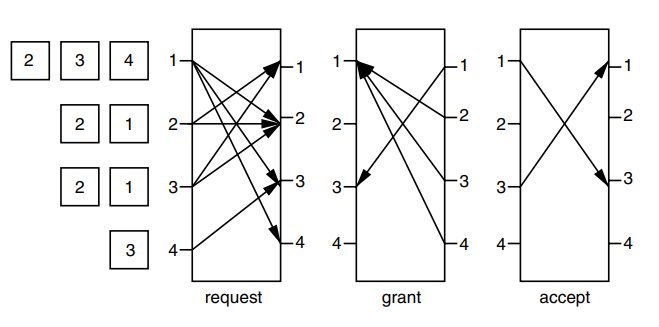
\includegraphics[width=1\textwidth]{imagem_islip.png}
  \caption[Iteração do iSLIP]{Iteração do iSLIP (fonte: \cite{math})}
  \label{fig:airbus1}
\end{figure}


Na fase de \textit{request}, o porto 1 requer o envio de tramas para os portos 2, 3, e 4; o porto 2 requer o envio para os portos 2 e 1; o porto 3 requer o envio para os portos 2 e 1; o porto 4 requer o envio para o porto 3. Na fase de \textit{grant}, o porto 1 oferece permissão de envio ao porto 3, enquanto os restantes portos oferecem permissão ao porto 1. Na fase de \textit{accept}, o porto 1, de entre as permissões que lhe são atribuídas decide transmitir para o porto 3, enquanto o porto 3 decide transmitir para o porto 1. Se o algoritmo acabar aqui, os portos 2 e 4 não têm opção de transmitir tramas, porque nenhum porto lhes deu essa permissão. Caso contrário, na iteração seguinte o algoritmo aumentará o \textit{match} correspondendo os portos de transmissão 2 e 4 relativamente aos portos de recepção 2 e 4.



Ao fim de uma iteração, nos portos de origem e destino que pertençam a uma correspondência, as listas de prioridades são atualizadas segundo a regra definida. Se o algoritmo estiver definido para uma iteração, a ronda acaba neste momento. Caso contrário, continua a tentar formar mais correspondências com os portos que ainda não pertençam a uma. Ao atualizar as listas de prioridade precisamente quando o respetivo porto fez parte de uma correspondência, a tendência a longo prazo será para haver dessincronização entre os elementos mais prioritários nas várias listas, reduzindo a ocorrência de exclusão de um porto no acesso à \textit{switch fabric}.


\section{Lógica de reencaminhamento}

No que diz respeito à tabela de endereços, dada a impossibilidade de utilizar uma memória CAM em FPGA, foi necessário pesquisar algoritmos de procura em tabelas implementados em \textit{hardware}. Numa análise exaustiva de alguns algoritmos, aplicados no contexto do protocolo HSR, foi encontrada uma solução \cite{HSR}. No documento são propostos três algoritmos para procurar e inserir elementos numa tabela.\par 
O primeiro algoritmo é denominado de "\textit{buffer} circular". Neste algoritmo, uma tabela é implementada juntamente com um ponteiro de escrita. De cada vez que é necessário escrever dados na tabela o ponteiro é incrementado. Excecionalmente, se o ponteiro se encontrar no fim da tabela, este volta para o início após uma escrita. Desta forma é garantido que as entradas da tabela que vão sendo retiradas são as mais antigas, permanecendo as mais recentes. A implementação desta solução é simples, no entanto, pode não ser a mais vantajosa se se desejar uma consulta da tabela consistentemente de curta duração. Em última análise, devido há falta de qualquer tipo de organização da tabela, será necessário percorrer toda a tabela para descobrir que um endereço não se encontra registado na mesma.\par 
Por forma a melhorar a eficiência temporal da procura na tabela, é analisado um segundo algoritmo com recurso a tabelas de dispersão. As tabelas de dispersão consistem em estruturas de dados que possuem alguma organização na distribuição da informação contida nos vários endereços de memória. Nestas tabelas, cada pedaço integral de informação que se pretende inserir ou procurar é mapeado através de uma função para um endereço de memória específico. Idealmente, as funções de dispersão devem ser totalmente aleatórias para reduzir a coincidência da função de dispersão de dois elementos diferentes, o que se denomina de colisão. No entanto, quando a quantidade de endereços de memória numa tabela não é várias ordens de grandeza maior que a quantidade de elementos possíveis de serem armazenados, as colisões tornam-se inevitáveis. Assim, torna-se necessário implementar técnicas que permitam manter presentes na tabela, em simultâneo, vários elementos que tenham sido mapeados para o mesmo endereço, e, posteriormente, aceder-lhes em momento de leitura. No estudo referido, foi implementada a técnica denominada \textit{Open Adressing}. Quando aplicada esta técnica, no momento de uma colisão, a procura pela informação pretendida continua para o endereço seguinte, segundo uma regra definida, até se encontrar os dados pretendidos ou se decida parar a procura. Por forma a não se dispensar demasiado tempo na procura, o autor definiu que a procura por um conjunto de dados estaria limitada a uma quantidade predefinida de endereços. Para finalizar o algoritmo, quando os dados não são encontrados nos endereços selecionados, os mesmos são inseridos no endereço cujo conteúdo foi mais antigamente acedido. Este algoritmo nunca procede a procuras tão lentas como o primeiro algoritmo poderá fazer, no entanto, a sua implementação é muito mais complexa devido ao mecanismo de rastreamento dos momentos de leitura das várias posições de memória.\par 
Por último, é proposto um algoritmo com a pretensão de ter uma eficiência semelhante ao segundo algoritmo, mas com uma complexidade de implementação semelhante ao primeiro algoritmo. Para isso, a tabela de endereços é divida num conjunto de \textit{buffers} circulares de reduzida dimensão, onde cada \textit{buffer} possui um ponteiro de escrita e um ponteiro de leitura. Tal como no segundo algoritmo, é aplicada uma função de dispersão. No entanto, esta mapeia os dados a procurar a um dos vários \textit{buffers} ao invés de a um endereçamento de memória. Após o mapeamento, o ponteiro de leitura é sucessivamente incrementado até que seja encontrado o que se procura ou se tenha percorrido a totalidade do \textit{buffer}. Quando não encontrados, os dados são guardados no endereço para o qual aponta o ponteiro de escrita, sendo este seguidamente incrementado. Quando a eficiência do algoritmo é medida como a probabilidade de serem encontrados na tabela os dados procurados, este algoritmo será teoricamente inferior ao anterior. A razão para isso prende-se com a escolha do endereço de memória a atualizar em caso de insucesso na procura. No segundo algoritmo, o endereço atualizado é aquele cujos dados permanecem hà mais tempo sem serem acedidos, face ao último endereço a ser escrito, que é a solução usada no terceiro algoritmo. 
\par Uma simulação em redes HSR de variada dimensão foi elaborada no estudo referido, onde foi validado o desempenho equiparável das duas variantes de tabela de dispersão. Assim, devido à maior simplicidade de implementação da tabela com recurso a um conjunto de \textit{buffers} circulares será essa a solução escolhida para operar como tabela de endereços.


